% \documentclass[main.tex]{subfiles} % Subfile-Class

\documentclass{article}
\usepackage{graphicx}
\usepackage{float}



% ============================================================================== %
%                            Subfile document                                    %
% ============================================================================== %

\begin{document}

% Template

% ===================================
\subsection{Evaluation eines Liniensensors}

Im folgenden Abschnitt ist die Entwicklung und Evaluierung eines Liniensensors
dokumentiert. Ziel ist es, einen einfach auszuwertenden Sensor zu entwickeln,
der das vorgegebene Klebeband vom Wettkampf-Untergrund unterscheiden kann.

% ===================================
\subsubsection{Anforderungen}
Es muss das Klebeband \textit{Tesa Gewebeband 4651} auf einem rötlich
gefliessten Untergrund detektiert werden. Eine besondere Herausforderung
stellen hierbei längs und quer verlaufende Fliesenfugen dar, welche eine
ähnliche Farbe aufweisen. Dieser Untergrund ist in
Abbildung~\ref{fig:Untergrund_Wettkampf} gezeigt.

\begin{figure}[H]
    \centering
    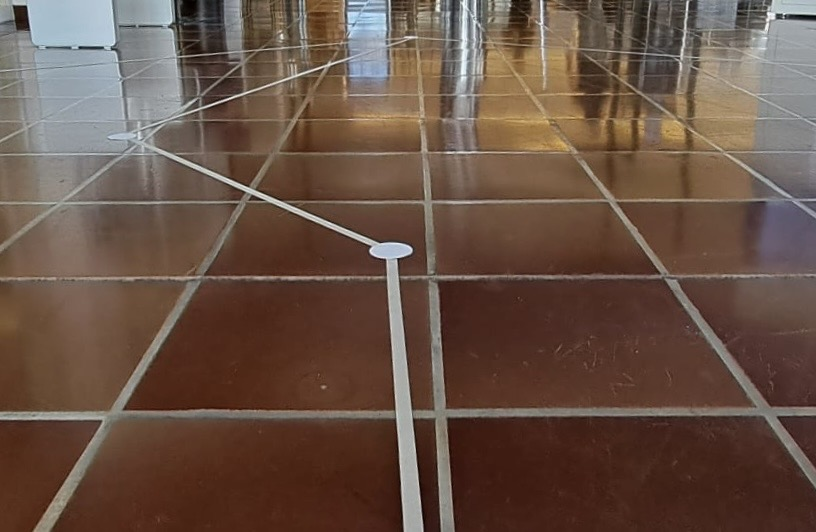
\includegraphics[width=0.75\textwidth]{Bild_Untergrund.jpg}
    \caption{Untergrund während des Wettkampfs}~\label{fig:Untergrund_Wettkampf}
\end{figure}

% ===================================
\subsubsection{Konzeption}
Dieser Versuch behandelt die Detektion der Linie anhand verschiedener
Lichtspektren. Als erstes wird die Linie im Infrarotspektrum bestrahlt und die
stärke der Reflektion an anhand eines Fototransistors, welcher ebenfalls im
Infrarotbereich sensitiv ist, auf einem Microcontroller ausgewertet. \

Als zweites wird die Linie im ultravioletten Bereich angestrahlt und im
sichtbaren Lichtspektrum ausgewertet. Ziel ist es, eine mögliche floureszierende Wirkung
des weissen Klebebands zu erfassen und auszuwerten.

% ===================================
\subsubsection{Entwicklung und Dimensionierung}

\paragraph{Geometrische Überlegungen}
Abbildung~\ref{fig:Konzept_graphml} zeigt konzeptionelle Überlegungen zum
Liniensensor. Ziel ist es, ein Array aus 8 Sender-Empfänger-Paaren
herzustellen, welches mindestens 2 Messzellen überhalb des Klebebandes besitzt. Diese
einzelnen Messzellen sollen untereinander und von der Umwelt abgekapselt sein. Dies
mit der Begründung, dass die Fototransistoren, (Empfänger), gegebenenfalls empfindlich auf
Umwelteinflüsse reagieren könnten. Das ausgewählte Sender-/Empfängerpaar
besitzt, sowohl bei den UV-, als auch bei den Infrarotbauteilen, einen
Abstrahlwinkel von 30°, beziehungsweise einen Einfallswinkel von 60°. Diese
Winkel und den festgelegten Abstand von Empfänger zu Sender definieren den
Abstand der Messzellen und den Abstand des Sender
und Empfänger-Paars vom Boden. Auf dem Boden muss eine möglichst grosse Fläche des Empfänger-Kreises 
durch den Sender-Kreis ausgefüllt werden.

\begin{figure}[H]
    \centering
    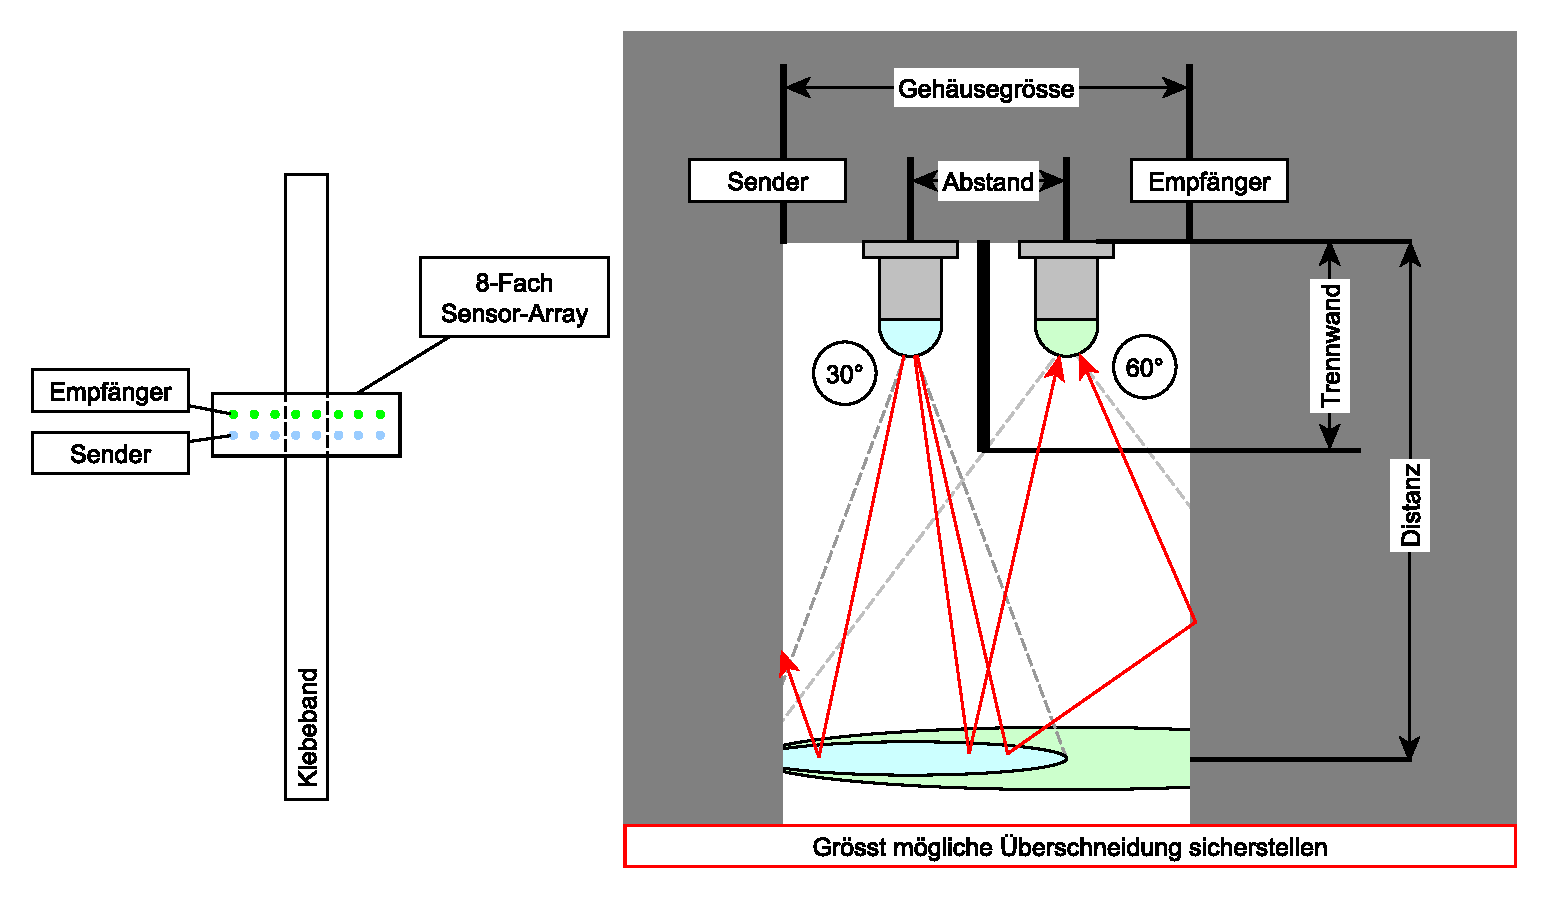
\includegraphics[width=0.75\textwidth]{Konzept.pdf}
    \caption{Konzept des Liniensensors}~\label{fig:Konzept_graphml}
\end{figure}


\paragraph{Dimensionierung der Position von Sender und Empfänger}
In diesem Abschnitt wird die optimale Positionierung der Sender und Empfänger ermittelt.\\ 
Der Abstand zwischen einem Sender und einem Empfänger wird aufgrund der Bauform beider 
Komponenten bestimmt.
Beide Komponenten besitzen das gleiche Gehäuse. Gemäss Datenblatt ist der Durchmesser
beider Komponenten mit Herstellertoleranz maximal 4mm. Es folgt eine Berechnung des 
Mindestabstand beider Komponenten. Das Mass bezieht sich auf die Mitte der beiden 
Komponenten, wie in Abbildung~\ref{fig:Konzept_graphml} dargestellt.
\[ X_{min} = \frac{D_s}{2} + \frac{D_e}{2} = \frac{4mm}{2} + \frac{4mm}{2} = 4\,\text{mm} \]
Damit genügend Reserve vorhanden ist, wird ein Abstand von 4.6mm zwischen Sender und
Empfänger in einer Messzelle gewählt.\\

Folglich wird der Abstand zwischen Sender/ Empfänger und Boden ermittelt. Dafür 
wird die Beziehung der beiden Radien ausgenutzt, welche bei der zu ermittelnden Höhe
h auf den Boden gestrahlt werden. Es folgt also:

\[
R_s = \tan(\alpha) \cdot h 
\]
\[
R_e = \tan(\beta) \cdot h
\]

Nun kann \( R_e \) auch durch \( R_s \) und den Mindestabstand \( X_{min} \) formuliert werden:
\[
    R_e = R_s + X_{min}
\]
Nun wird \( R_s \) und \( R_e \) eingesetzt und nach h aufgelöst:
\[
h = \frac{4.6}{\tan(\beta) - \tan(\alpha)} = \frac{4.6mm}{\tan(30^\circ) - \tan(15^\circ)} = 14.867{mm} \approx 15{mm}
\]
Aus der Höhe h kann nun der Abstand von zwei Messzellen berechnet werden. Dafür 
wird zuerst der Radius \( R_s \) des Senders berechnet:
\[
R_s = \tan(\alpha) \cdot h = \tan(15^\circ) \cdot 14.867{mm} = 3.984{mm} \approx 4{mm}
\]
Der Abstand von zwei Messzellen, von Mitte zu Mitte, beträgt dementsprechend:
\[
X_{zellen} = 2 \cdot R_s + X_{trenn} = 2 \cdot 4{mm} + 1{mm} = 9{mm}
\]
Mit dem \( X_{trenn} \) wurde ein Trennabstand von 1mm einberechnet. Dieser 
Sicherheitsabstand sorgt, das kein Schnittpunkt zwischen zwei Messzellen entsteht.

\paragraph{Dimensionierung Gehäuse}
Damit der Empfänger möglichst wenig auf Umwelteinflüsse reagiert, wird nun ein 
Gehäuse dimensioniert, welches den Sensor abschirmen soll. Die nachfolgende 
Abbildung~\ref{fig:Skizze_Gehause} zeigt eine Skizze, welche den Aufbau des Gehäuses repräsentiert.

!!!! SKIZZE AUFBAU TRENNWÄNDE !!!!\\
!!!!! dies ist lediglich ein Platzhalter !!!!!
\begin{figure}[H]
    \centering
    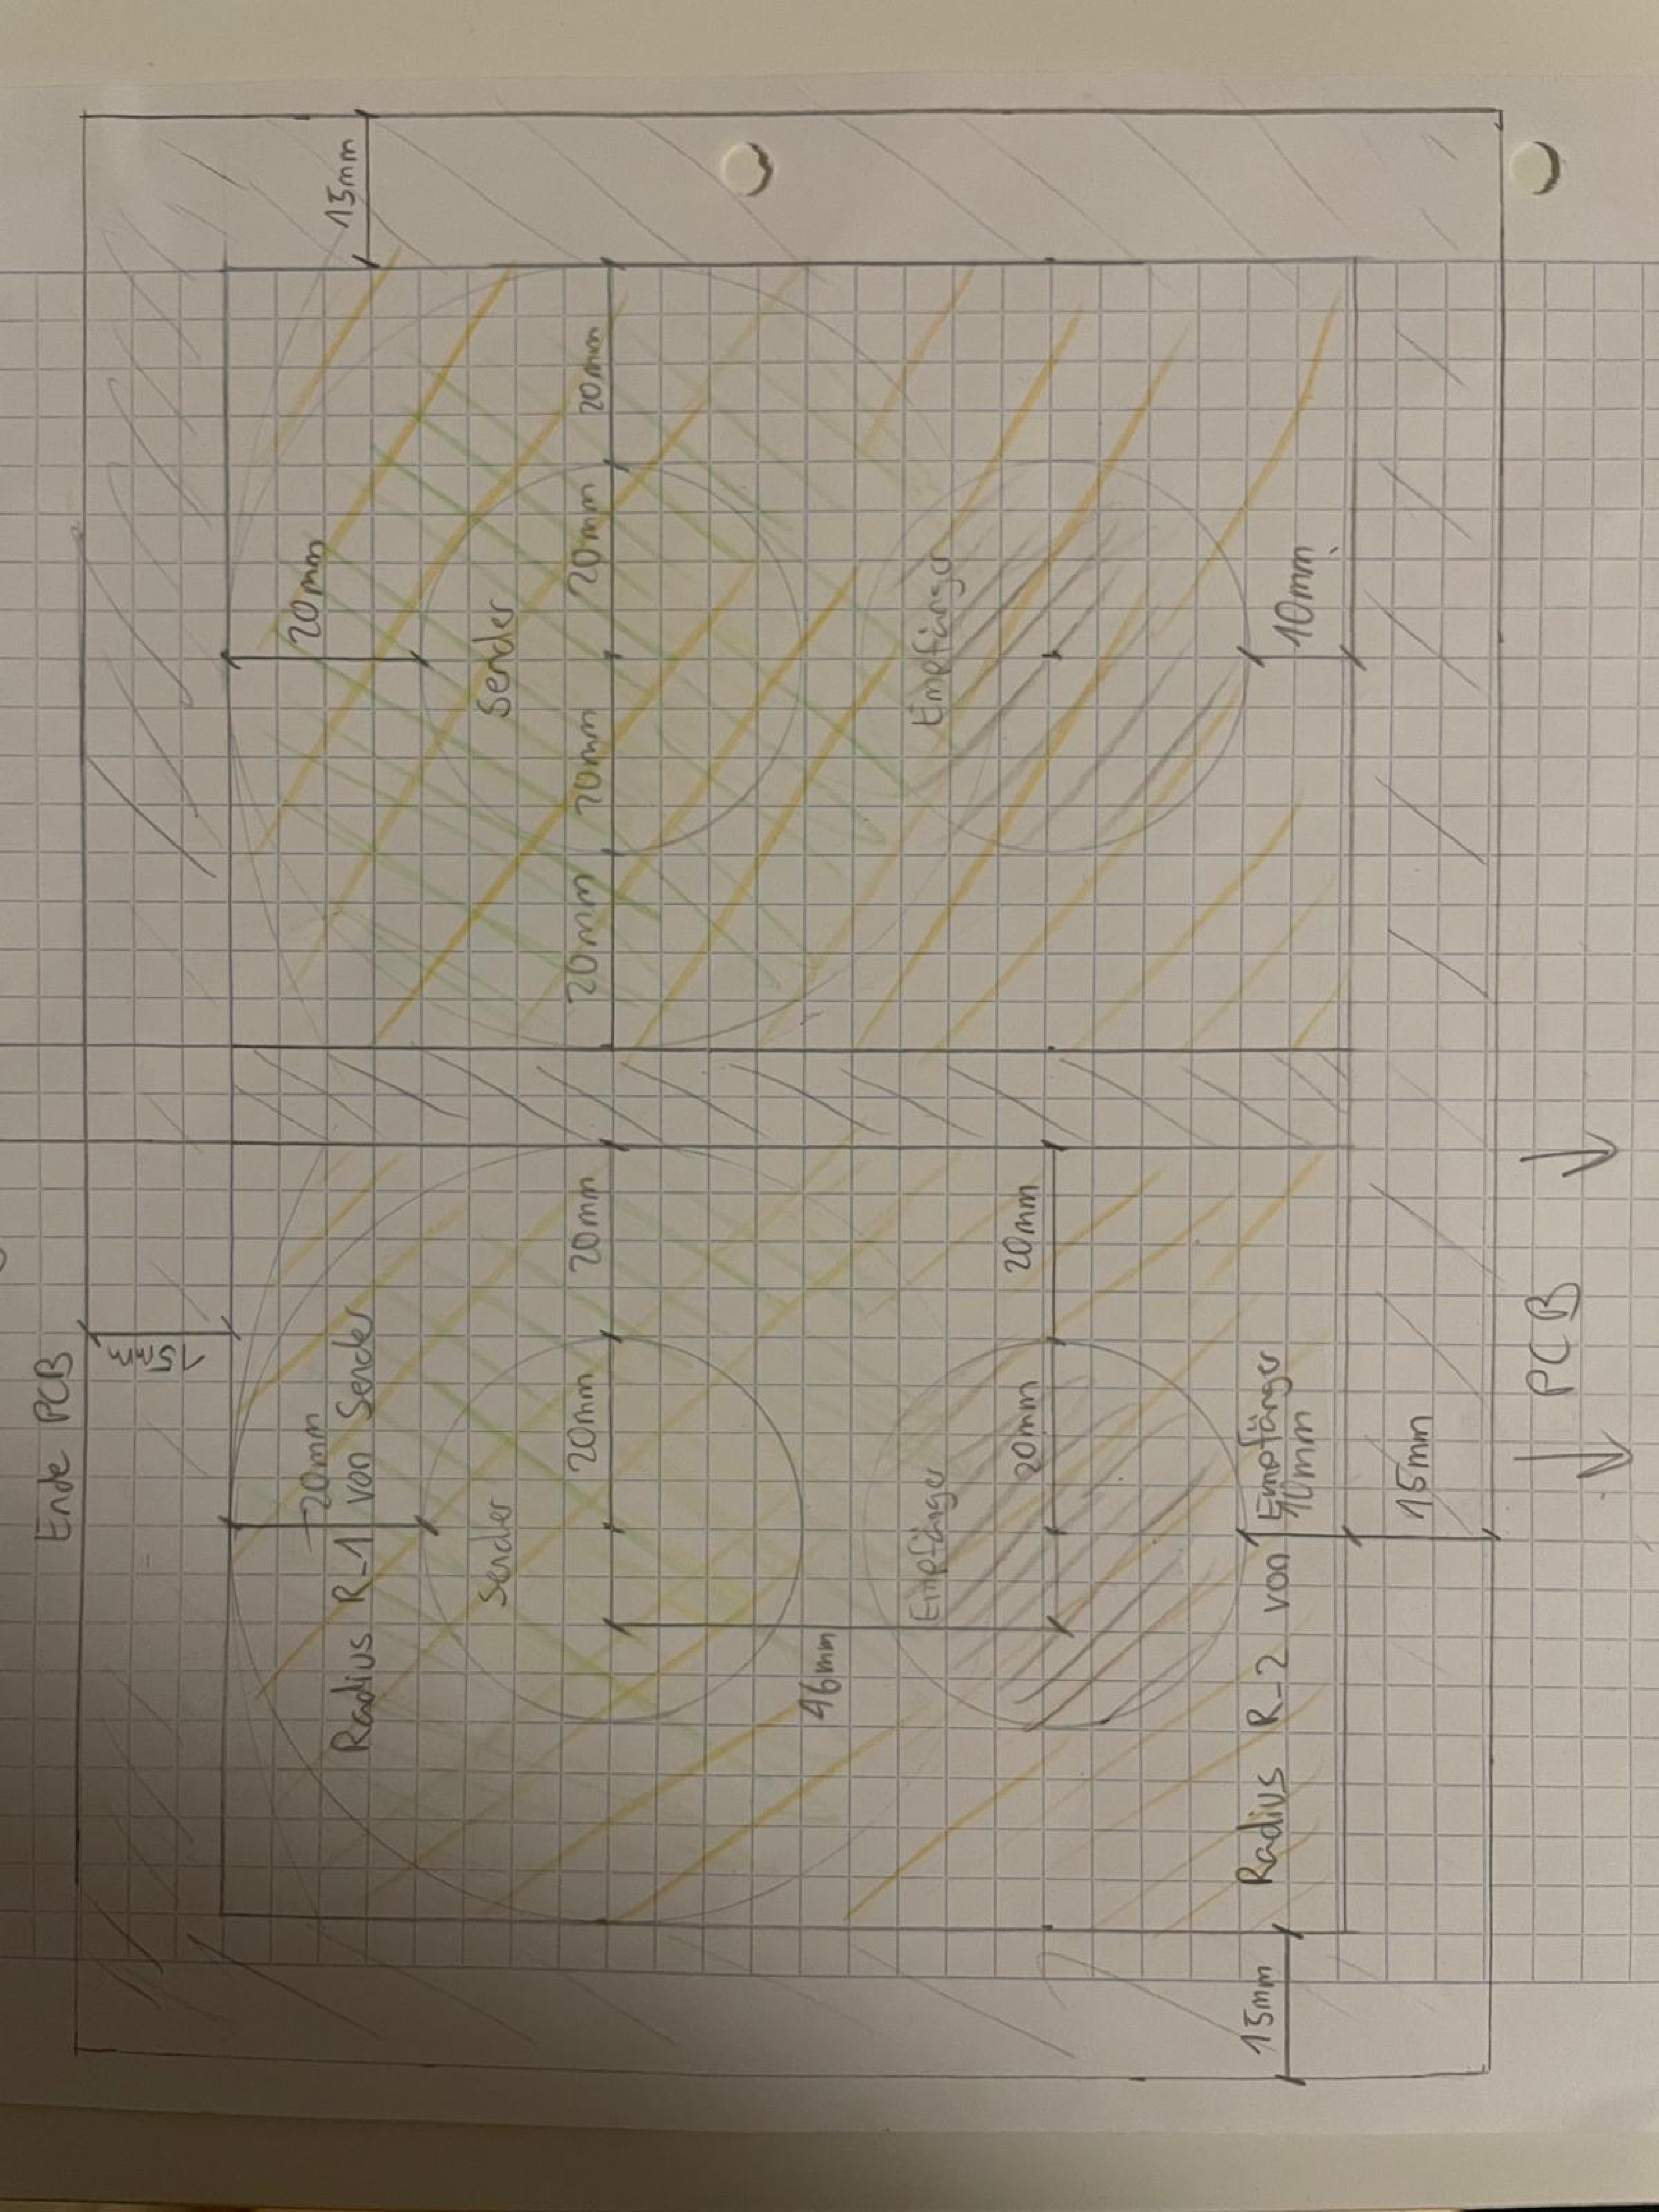
\includegraphics[width=0.5\textwidth]{Skizze_Gehause_oben.pdf}
    \caption{Skizze des Gehäuse von oben}~\label{fig:Skizze_Gehause}
\end{figure}

In der Skizze aus Abbildung XY sind die Radien \(R_s\) und \(R_e\) ersichtlich, welche 
von dem Sender und Empfänger auf den Boden projeziert werden. Diese Radien werden durch 
die Trennwände des Gehäuses begrenzt. Der Radius \(R_s\) ist daher massgebend für die 
Vermassung von drei der vier Wände des Gehäuses. Der Abstand des Mittelpunktes des 
Empfängers zu der untersten Wand beträgt 3mm. Es wurde 1mm als Reserve zwischen 
Bauteil und Wand einberechnet. Die Wandstärke der Trennwände zwischen den Sensorzellen
wurden auf 1mm und die Aussenwände auf 1.5mm (NOCH NICHT DEFINITIV!) festgelegt. 
Die Wandstärken wurden absichtlicht so geplant, damit sie möglichst dünn ausfallen 
aber dennoch im 3D-Drucker realisierbar sind. Die Höhe des Gehäuse wird 14mm hoch, 
damit es ungefähr einen Millimeter kleiner ist, als die oben berechnete Höhe h von 
Sensor zu Boden.



\paragraph{Elektrotechnische Überlegungen}

\begin{figure}[H]
    \centering
    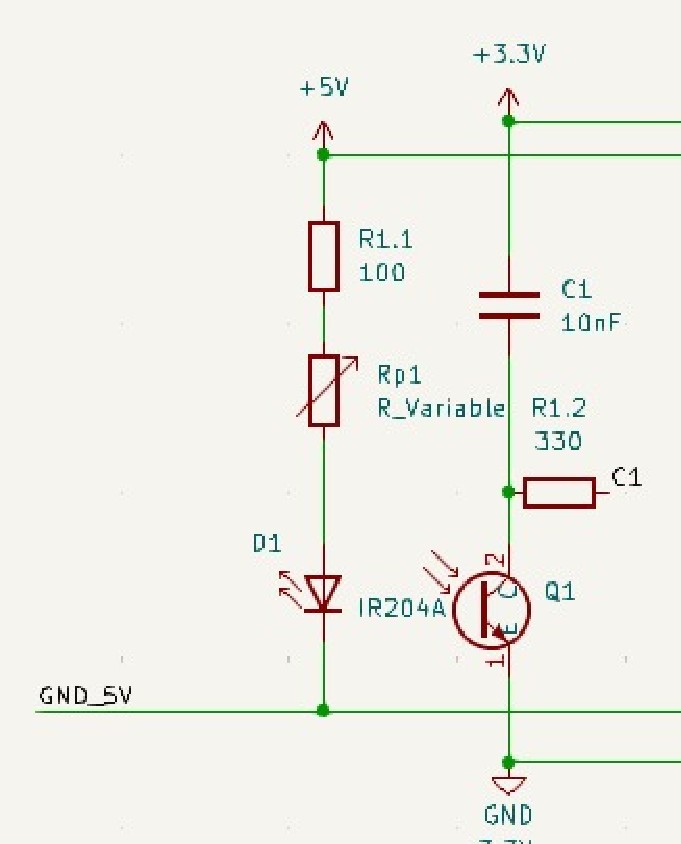
\includegraphics[width=0.5\textwidth]{Schema_Sensorzelle.pdf}
    \caption{Schema einer Sensorzelle}~\label{fig:Sensorzelle}
\end{figure}


!!! SCHEMA MANU EINSETZEN !!!


Abbildung~\ref{fig:Sensorzelle} zeigt das Schema einer einzelnen Sensorzelle.
Über die Speisespannung wird eine LED bestromt, deren Vorwiderstand sich wie
folgt berechnet:

\[
    R_{LED} = \frac{Uq - Uv}{I_{LED}}
\]

$Uv$ beträgt bei der UV-LED laut Datenblatt $3.2V$, weshalb hier die Speisespannung
auf 5V angehoben werden muss. Deshalb wird bei der Dimensionierung für den Vorwiderstand
auch mit 5V Quellspannung gerechnet, wohingegen der Fototransistor für den Microntroller
auf $3.3V$ arbeitet.

Der Vorwiderstand der Sende-LED wird auf $I=20mA$ ausgelegt und ein
zusätzliches Potentiometer vorgeschaltet, welches ein genaues Trimmen auf
$10...20mA$ Diodenstrom und damit ein einstellen der Leuchtstärken erlaubt.
Damit können auch Bauteiltoleranzen in den Fototransistoren und Kondensatoren
ausgeglichen werden. \\

Der Fototransistor an sich wird für die Berechnung als Konstantstromquelle
betrachtet, wobei sich die Kapazität des Kondensators wie folgt ergibt.

\[
    Q = C \cdot U \qquad \& \qquad I = \frac{Q}{t}
\]

\[
    C = \frac{I \cdot t}{U}
\]

Bei einer angenommenen Entladezeit von $t = 30us$, einem Mindeststrom von $1
    mA$ und einer Versorungsspannung von $U_q = 3.3V$ ergibt sich eine Kapazität
von ca. $10nF$. Der GPIO des Microcontrollers muss ebenfalls durch einen
Vorwiderstand im Strom begrenzt werden. Im Datenblatt des Raspberry Pico ist ein
maximaler Strom von $10 mA$ als Maximalwert angegeben. Ein entsprechender
Vorwiderstand beläuft sich demzufolge laut dem ohm'schem Gesetz zu

\[
    R = \frac{U}{I} = \frac{3.3V}{10mA} = 330 \Omega
\]

Der Kondensator muss also mindestens $5 \cdot \tau$ entladen werden. Das bringt
die folgende Zeit.

\[
    t_{laden} > 5 \cdot \tau = 5 \cdot RC = 5 \cdot 330 \Omega \cdot 10nF = 16us
\]

Der Kondensator muss beim Abfragen also mindestens $16us$, besser mindestens
$20 us$ geladen werden, bevor er ausgewertet wird.

\begin{figure}[H]
    \centering
    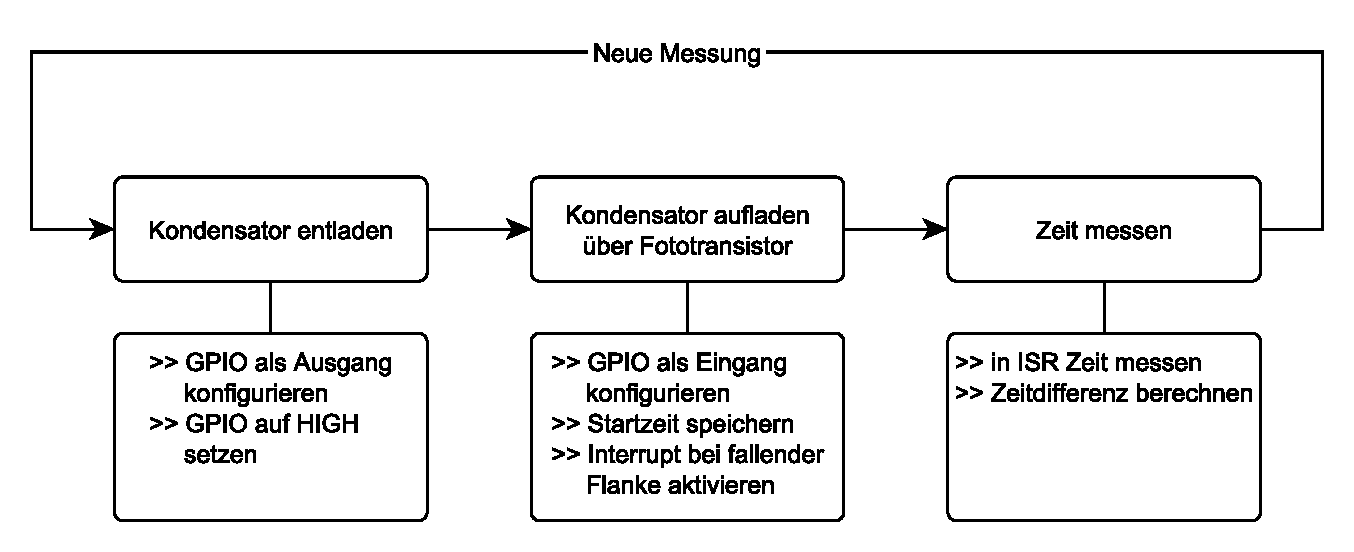
\includegraphics[width=0.75\textwidth]{Auswertung.pdf}
    \caption{Auswertung des Liniensensors}~\label{fig:Auswertung_Liniensensor}
\end{figure}


% ===================================
\subsubsection{Liniensensor als PCB}
\paragraph{Entwerfung des PCB}Damit der Liniensensor möglichst praxisnahe getestet 
werden kann, wurde dieser als PCB mit dem CAD-Tool Kicad erstellt. Dabei wurden die 
oben formulierten Anforderungen und Dimensionierungen eingehalten. In Abbildung~\ref{fig:Liniensensor_Top} 
ist die Draufsicht und in Abbildung~\ref{fig:Liniensensor_Bottom} die Untersicht dargestellt. Des Weiteren ist 
das Gehäuse für die Abschirmung von Umwelteinflüssen dargestellt. In Abbildung~\ref{fig:Gehaeuse_Isometrisch} 
ist die isometrische Ansicht des Gehäuses dargestellt und die Abbildung~\ref{fig:Gehaeuse_Vermasst} zeigt das 
Gehäuse von oben mit den wichtigsten Massangaben.

\begin{figure}[H]
    \centering
    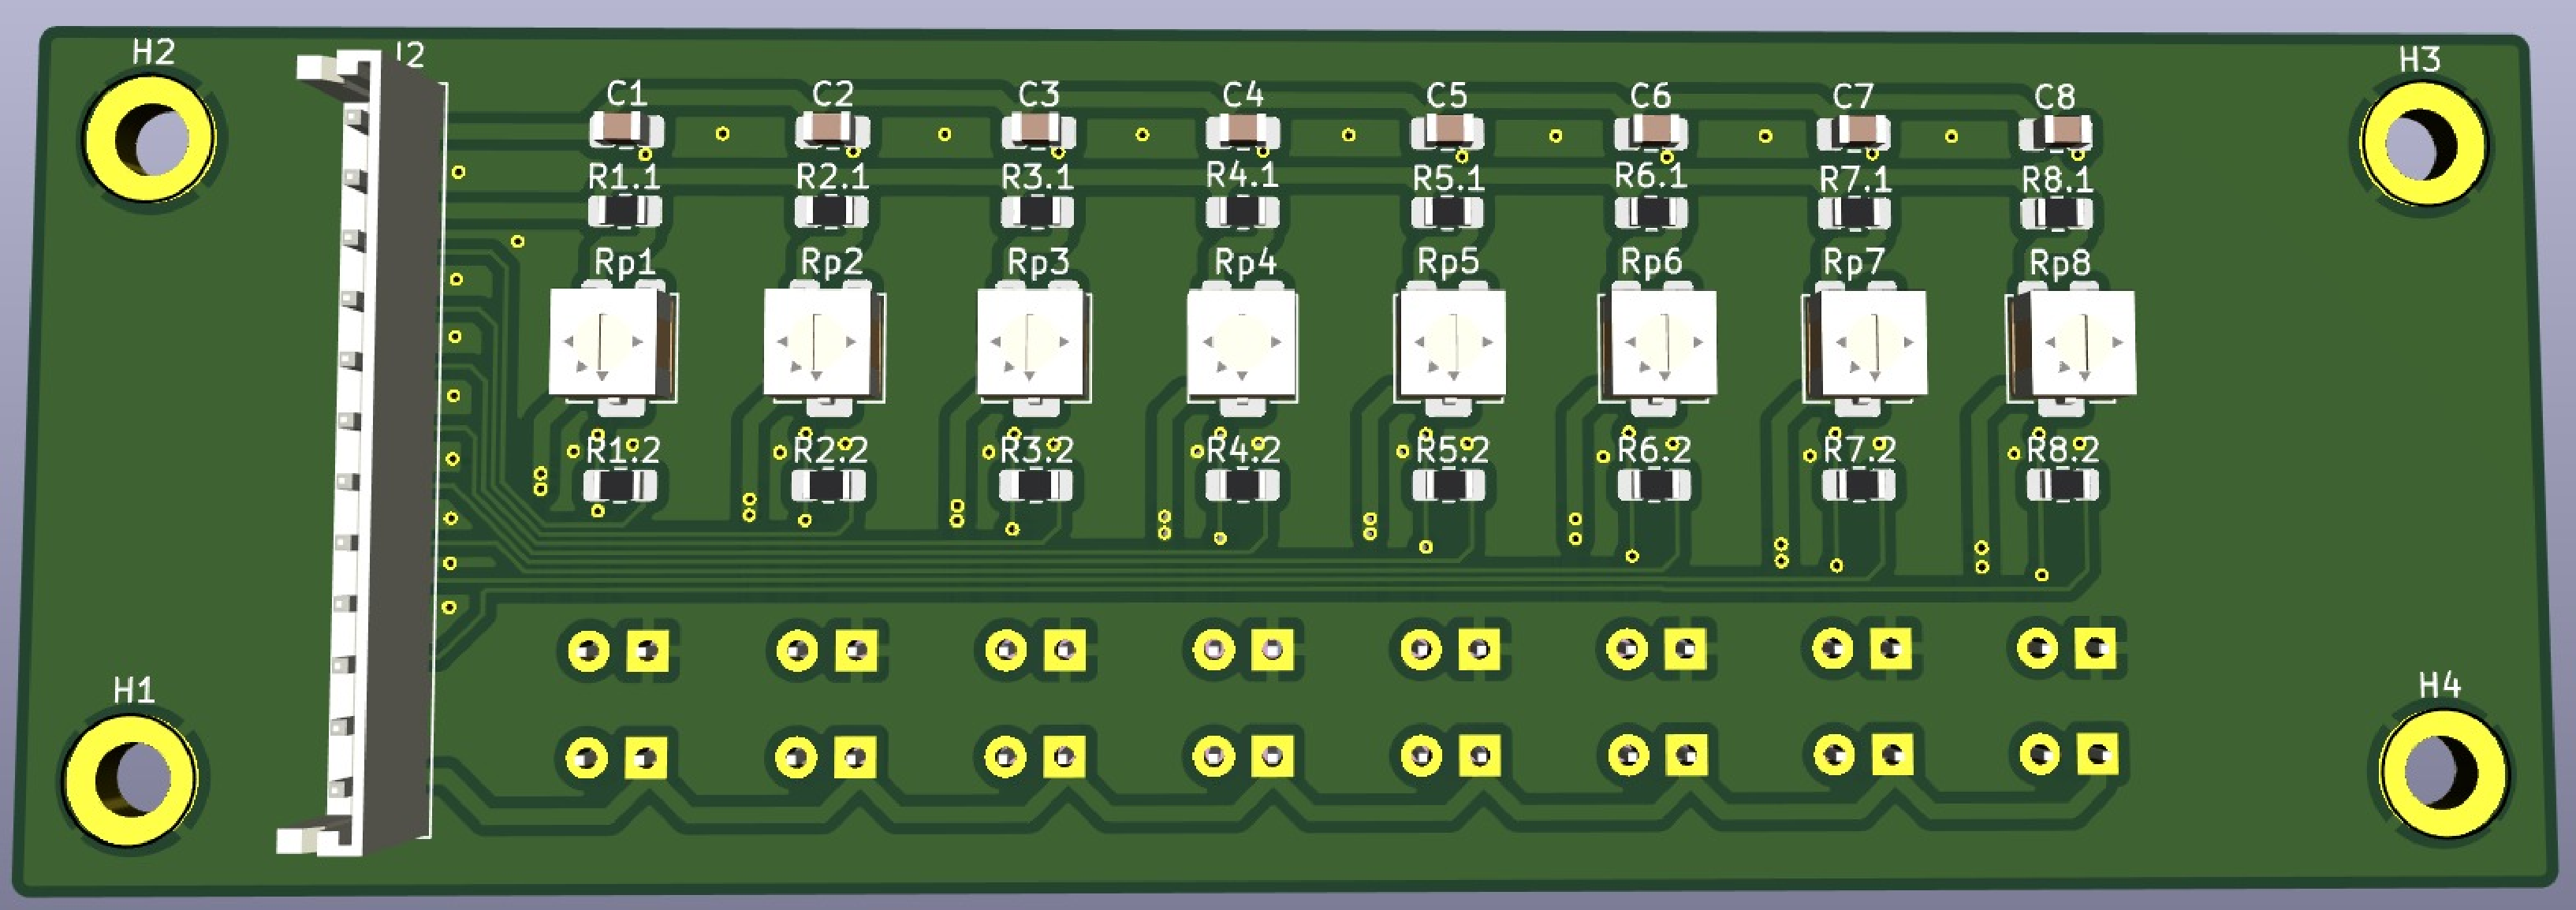
\includegraphics[width=0.75\textwidth]{Liniensensor_Top.pdf}
    \caption{Liniensensor in Kicad von oben}~\label{fig:Liniensensor_Top}
\end{figure}

\begin{figure}[H]
    \centering
    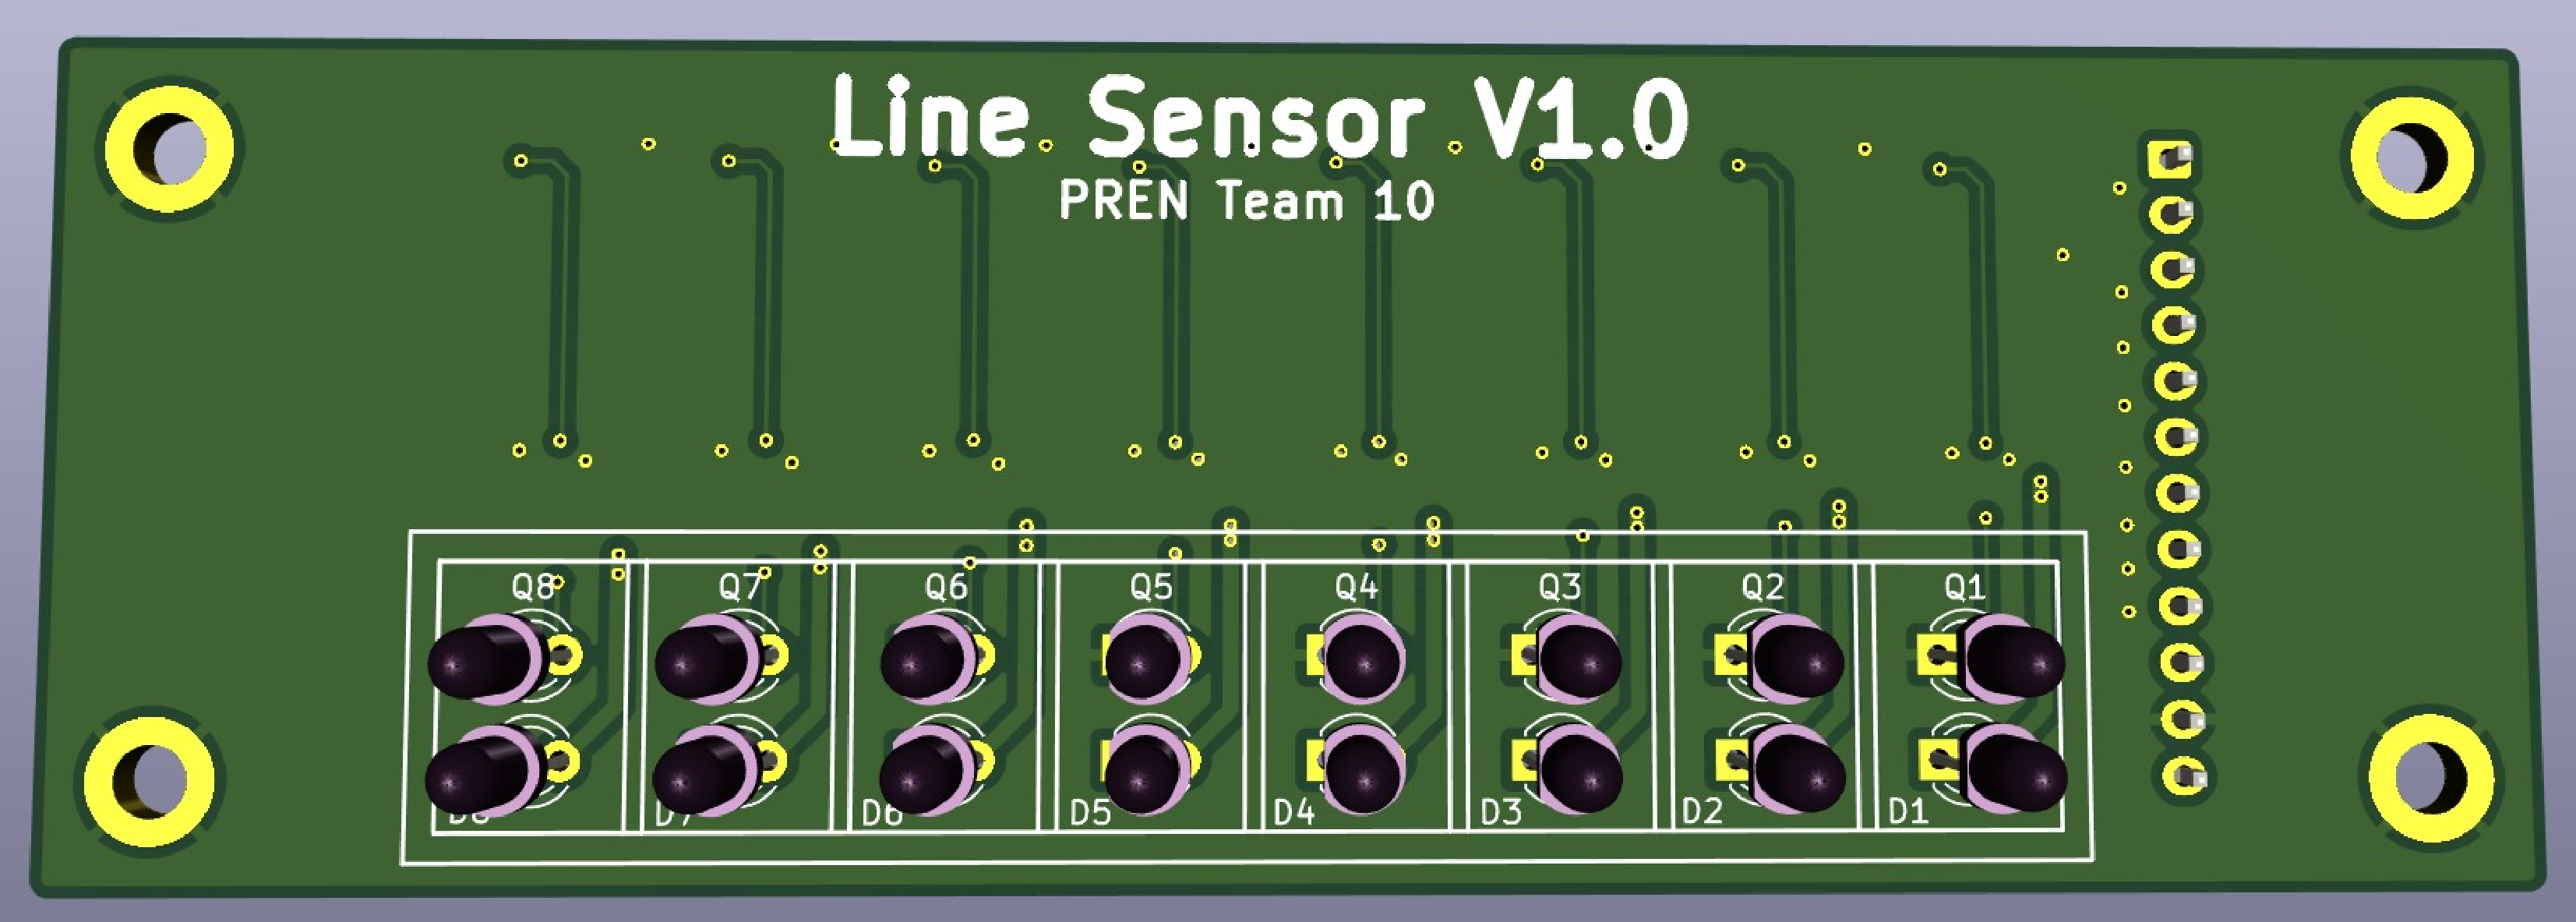
\includegraphics[width=0.75\textwidth]{Liniensensor_Bottom.pdf}
    \caption{Liniensensor in Kicad von unten}~\label{fig:Liniensensor_Bottom}
\end{figure}

\begin{figure}[H]
    \centering
    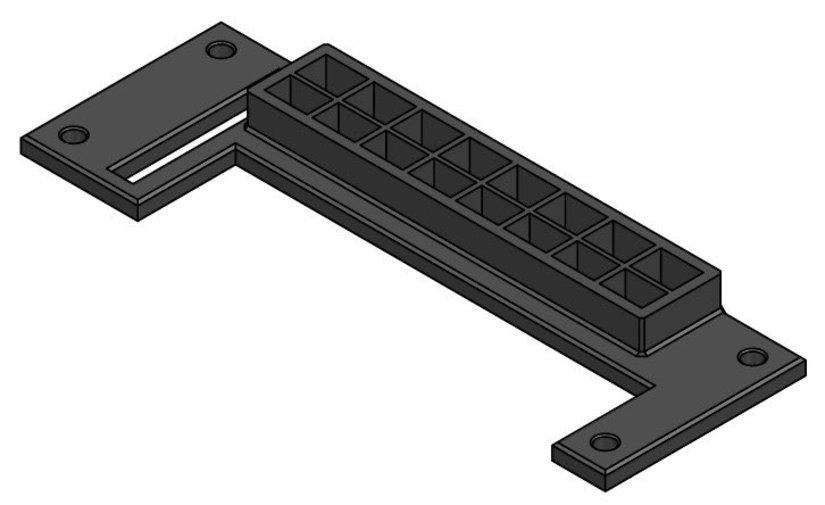
\includegraphics[width=0.75\textwidth]{Gehaeuse_Isometrisch.pdf}
    \caption{Isometrische Ansicht des Gehäuses in Siemens NX}~\label{fig:Gehaeuse_Isometrisch}
\end{figure}

\begin{figure}[H]
    \centering
    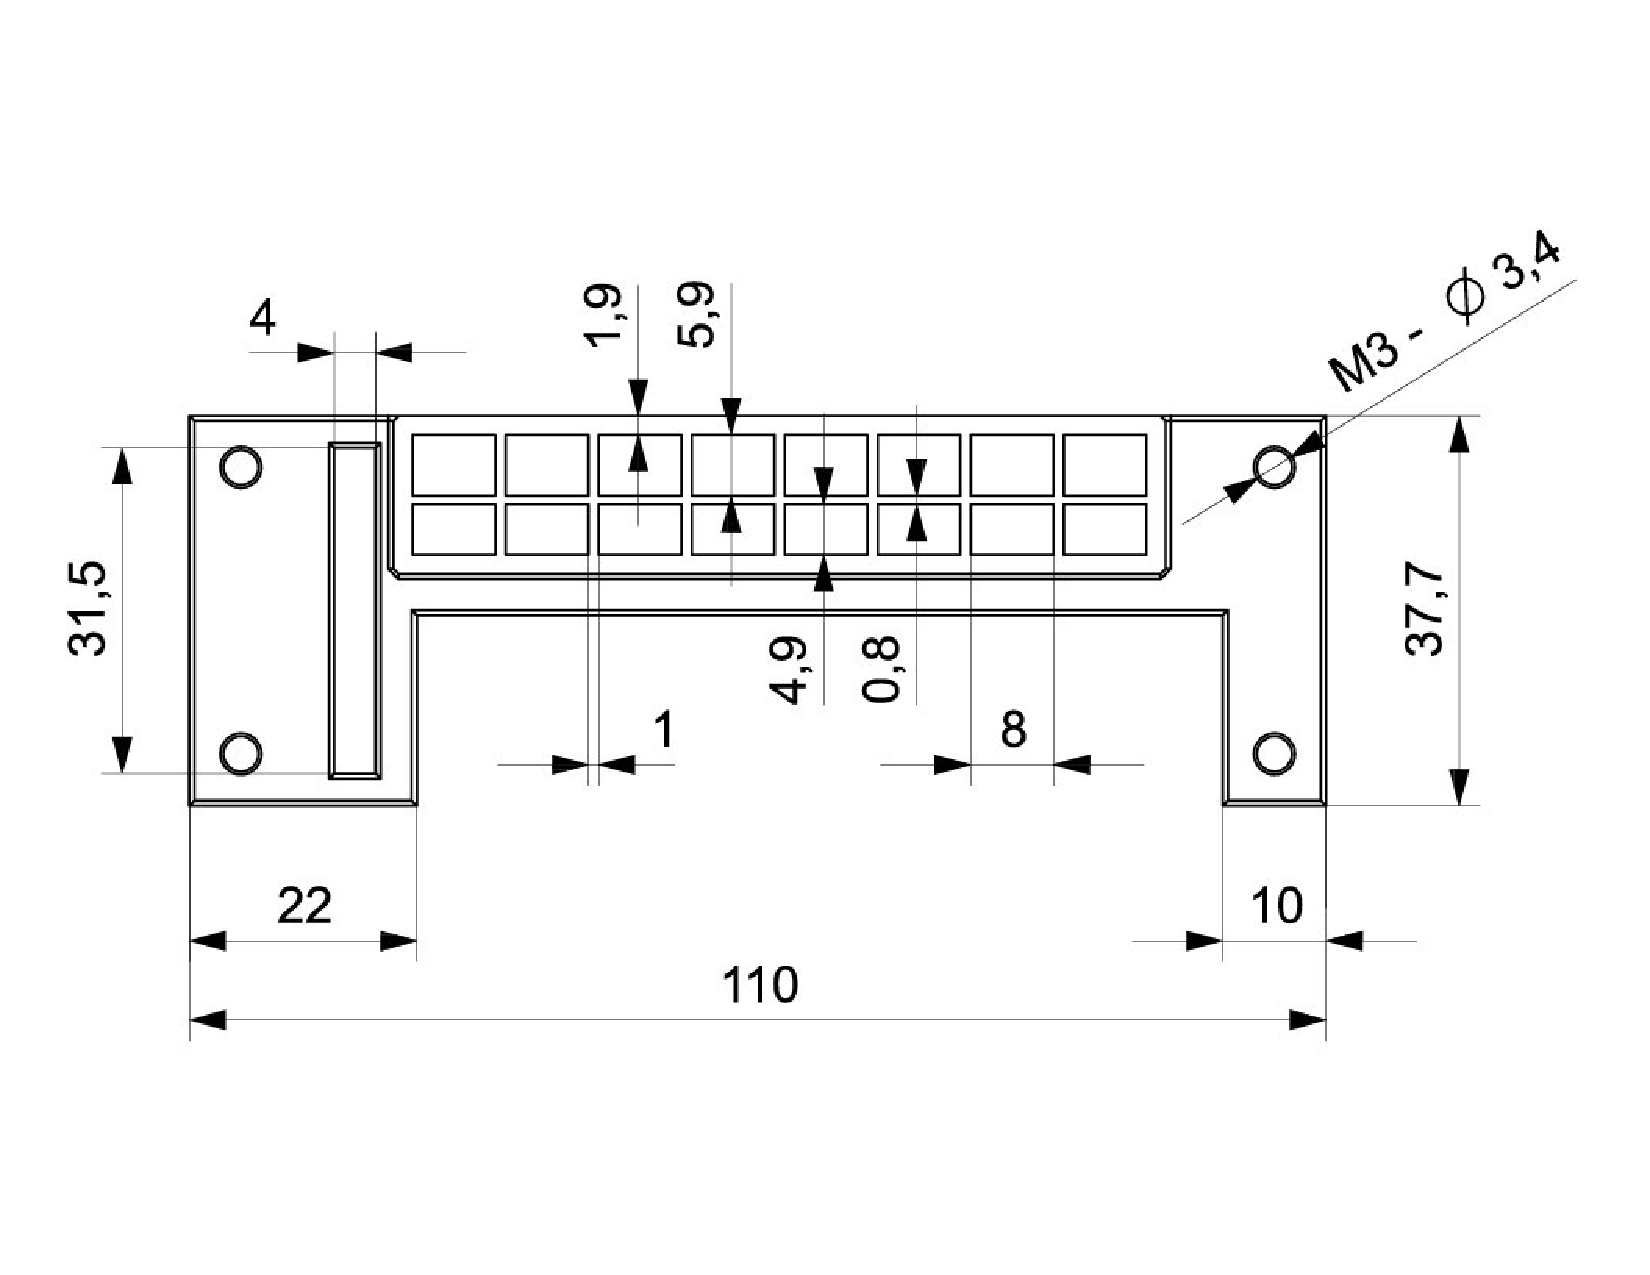
\includegraphics[width=0.75\textwidth]{Gehaeuse_Vermasst.pdf}
    \caption{Vermassung des Gehäuses in Siemens NX}~\label{fig:Gehaeuse_Vermasst}
\end{figure}

% ===================================
\subsubsection{Versuche}

% ===================================
\subsubsection{Fazit und Ausblick}

% ===================================

\end{document}
